\documentclass[11pt]{article}

\usepackage[margin=1.7cm]{geometry}
\usepackage{amsmath}
\usepackage{amssymb}
\usepackage{enumitem}
\usepackage{titlesec}
\usepackage{xcolor}
\usepackage{fancyhdr}
\usepackage{tikz}
\usetikzlibrary{arrows.meta}
\usepackage{pgfplots}
\usepackage{multicol}
\usepackage{array}
\pgfplotsset{compat=1.18}

\titleformat{\section}{\large\bfseries}{\thesection}{0.6em}{}
\titlespacing{\section}{0pt}{1.1em}{0.5em}

\pagestyle{fancy}
\fancyhf{}
\fancyhead[L]{Year 9 Algebra Revision --- Combining the Skills}
\fancyhead[R]{Name: \makebox[4cm]{\hrulefill}}
\fancyfoot[C]{\thepage}
\renewcommand{\headrulewidth}{0.4pt}

\newcommand{\ans}{\hrulefill}
\setlist[enumerate,1]{leftmargin=1.4em, itemsep=0.6em, topsep=0.2em}
\setlist[enumerate,2]{leftmargin=1.3em, itemsep=0.4em, topsep=0.2em}
\setlength{\columnsep}{1.1cm}
\setlength{\columnseprule}{0.4pt}

\newcommand{\markpt}[3]{\filldraw (axis cs:#1,#2) circle (1.5pt); \node[#3, font=\small] at (axis cs:#1,#2) {$(#1,#2)$};}
\newcommand{\dotpt}[2]{\filldraw (axis cs:#1,#2) circle (1.5pt);}

% \gridaxis{xmin}{xmax}{ymin}{ymax}{xtick dist}{ytick dist} -- axis lines through the origin
\newcommand{\gridaxis}[6]{%
  \begin{axis}[
    width=7.2cm, height=6.4cm,
    xmin=#1, xmax=#2, ymin=#3, ymax=#4,
    grid=both, grid style={line width=.1pt, draw=gray!35},
    axis lines=middle,
    xlabel={$x$}, ylabel={$y$},
    xtick distance=#5, ytick distance=#6,
    tick label style={font=\tiny},
    label style={font=\small},
    xlabel style={at={(axis description cs:1,0)}, anchor=north west},
    ylabel style={at={(axis description cs:0,1)}, anchor=south east},
    axis line style={-{Latex[length=1.8mm]}},
  ]
}

\begin{document}

\begin{center}
  {\Large\bfseries Year 9 Algebra Revision --- Combining the Skills}
\end{center}
\vspace{0.3em}
\noindent\textit{Each question now uses more than one skill. Show every step of your working.}

\vspace{0.4em}
\section{Simplify, then Solve}

\begin{multicols}{2}
\subsection*{Collect like terms, then solve}
\begin{enumerate}
  \item $3x + 2x - 1 = 14$ \ans
  \item $5x - 3 - x = 13$ \ans
  \item $2x + 3x + 4 = 24$ \ans
\end{enumerate}

\subsection*{Expand the bracket, then solve}
\begin{enumerate}[resume]
  \item $2(x + 3) = 16$ \ans
  \item $4(x - 2) = 8$ \ans
  \item $3(x + 1) = 21$ \ans
\end{enumerate}
\end{multicols}

\section{From a Pattern to a Line}
\noindent For each pattern: look at the diagrams, complete the table, write the rule, plot the points and draw the line, then state the gradient and $y$-intercept.

\begin{center}
\textbf{Squares made from matchsticks}

\vspace{0.4em}
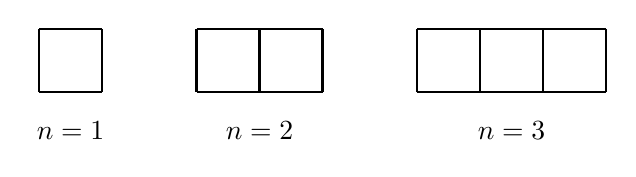
\begin{tikzpicture}[scale=0.8, line width=1pt]
  \draw (0,0) grid (1,1);
  \node[below] at (0.5,-0.3) {$n=1$};
  \begin{scope}[xshift=2.5cm]
    \draw (0,0) grid (2,1);
    \node[below] at (1,-0.3) {$n=2$};
  \end{scope}
  \begin{scope}[xshift=6cm]
    \draw (0,0) grid (3,1);
    \node[below] at (1.5,-0.3) {$n=3$};
  \end{scope}
\end{tikzpicture}

\vspace{0.6em}
\begin{tabular}{|c|c|c|c|c|c|}
\hline
$n$ (squares) & $1$ & $2$ & $3$ & $4$ & $5$ \\\hline
matchsticks & $4$ & $7$ & $10$ & & \\\hline
\end{tabular}

\vspace{0.4em}
How many matchsticks are added each time a new square joins the row? \ans

\vspace{0.6em}
Rule: matchsticks $=$ \ans
\end{center}

\begin{center}
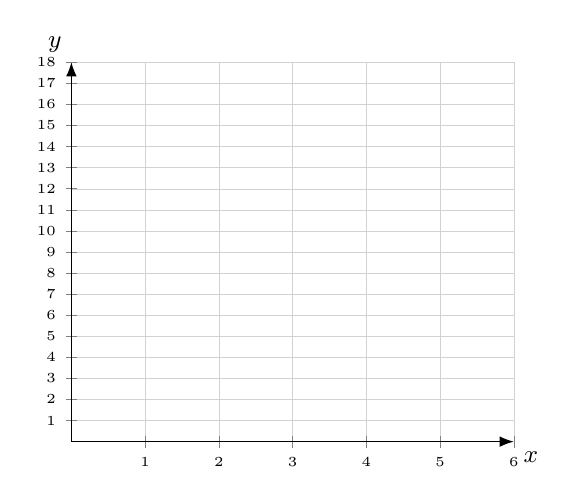
\begin{tikzpicture}
\gridaxis{0}{6}{0}{18}{1}{1}
\end{axis}
\end{tikzpicture}
\end{center}

\noindent Gradient: \ans \qquad\qquad $y$-intercept: \ans

\newpage
\begin{center}
\textbf{Triangles made from matchsticks}

\vspace{0.4em}
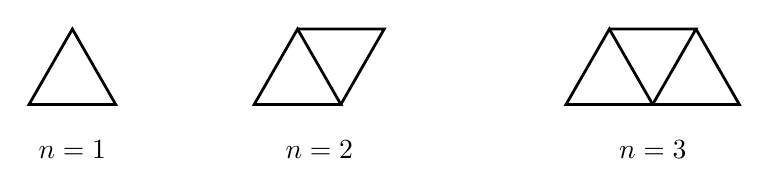
\begin{tikzpicture}[scale=1.1, line width=1pt]
  \draw (0,0) -- (1,0) -- (0.5,0.87) -- cycle;
  \node[below] at (0.5,-0.3) {$n=1$};
  \begin{scope}[xshift=2.6cm]
    \draw (0,0) -- (1,0) -- (0.5,0.87) -- cycle;
    \draw (0.5,0.87) -- (1.5,0.87) -- (1,0);
    \node[below] at (0.75,-0.3) {$n=2$};
  \end{scope}
  \begin{scope}[xshift=6.2cm]
    \draw (0,0) -- (1,0) -- (0.5,0.87) -- cycle;
    \draw (0.5,0.87) -- (1.5,0.87) -- (1,0);
    \draw (1,0) -- (2,0) -- (1.5,0.87);
    \node[below] at (1,-0.3) {$n=3$};
  \end{scope}
\end{tikzpicture}

\vspace{0.6em}
\begin{tabular}{|c|c|c|c|c|c|}
\hline
$n$ (triangles) & $1$ & $2$ & $3$ & $4$ & $5$ \\\hline
matchsticks & $3$ & $5$ & $7$ & & \\\hline
\end{tabular}

\vspace{0.4em}
How many matchsticks are added each time a new triangle joins the row? \ans

\vspace{0.6em}
Rule: matchsticks $=$ \ans
\end{center}

\begin{center}
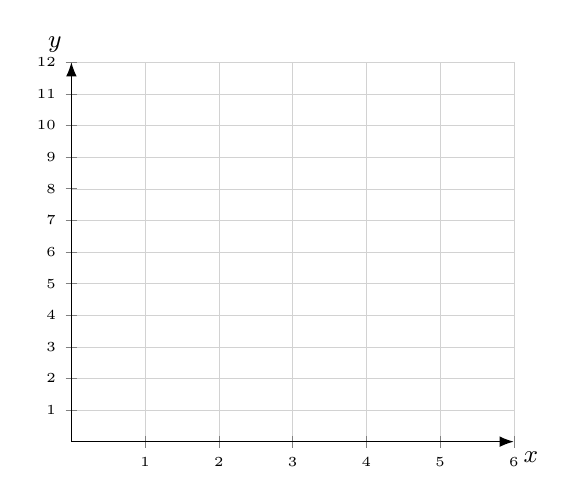
\begin{tikzpicture}
\gridaxis{0}{6}{0}{12}{1}{1}
\end{axis}
\end{tikzpicture}
\end{center}

\noindent Gradient: \ans \qquad\qquad $y$-intercept: \ans

\section{Using a Line's Equation}
\noindent Use substitution for part (a), then solve an equation for part (b).

\begin{enumerate}
  \item A line has equation $y = 2x + 5$.
  \begin{enumerate}
    \item Find $y$ when $x = 3$. \ans
    \item Find $x$ when $y = 17$. \ans
  \end{enumerate}

  \item A line has equation $y = -3x + 4$.
  \begin{enumerate}
    \item Find $y$ when $x = -2$. \ans
    \item Find $x$ when $y = -11$. \ans
  \end{enumerate}
\end{enumerate}

\newpage
\section{Finding the Equation from Two Points}
\noindent Each graph shows two points on a line, but the $y$-intercept is not marked. Find the gradient from the two points, then substitute one point into $y = mx + c$ to find $c$.

\begin{center}
\begin{minipage}{0.47\linewidth}
\centering
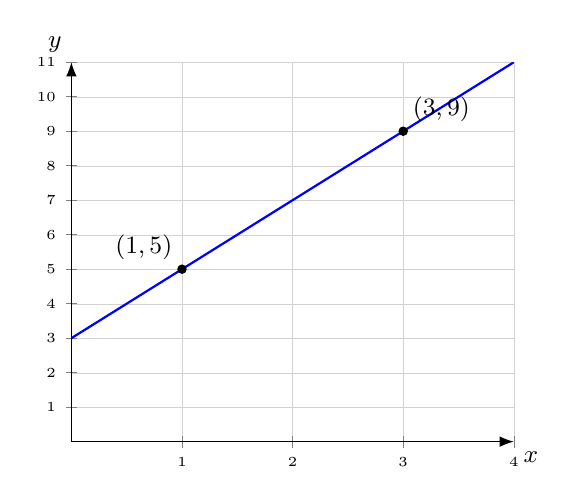
\begin{tikzpicture}
\gridaxis{0}{4}{0}{11}{1}{1}
\addplot[domain=0:4, samples=2, thick, blue] {2*x+3};
\markpt{1}{5}{above left}
\markpt{3}{9}{above right}
\end{axis}
\end{tikzpicture}

\vspace{0.3em}
Gradient: \ans \\[0.4em]
Equation: \ans
\end{minipage}
\hfill
\begin{minipage}{0.47\linewidth}
\centering
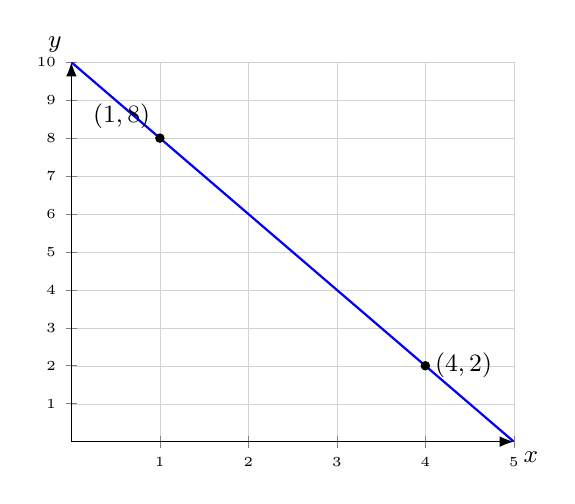
\begin{tikzpicture}
\gridaxis{0}{5}{0}{10}{1}{1}
\addplot[domain=0:5, samples=2, thick, blue] {-2*x+10};
\markpt{1}{8}{above left}
\markpt{4}{2}{right}
\end{axis}
\end{tikzpicture}

\vspace{0.3em}
Gradient: \ans \\[0.4em]
Equation: \ans
\end{minipage}
\end{center}

\section{Gradient and Equation from a Table}
\noindent For each table, find the gradient and $y$-intercept, then write the equation in the form $y=mx+c$.

\begin{center}
\begin{minipage}{0.47\linewidth}
\centering
\begin{tabular}{|c|c|c|c|c|}
\hline
$x$ & $0$ & $1$ & $2$ & $3$ \\\hline
$y$ & $1$ & $4$ & $7$ & $10$ \\\hline
\end{tabular}

\vspace{0.6em}
Gradient: \ans \\[0.4em]
$y$-intercept: \ans \\[0.4em]
Equation: \ans
\end{minipage}
\hfill
\begin{minipage}{0.47\linewidth}
\centering
\begin{tabular}{|c|c|c|c|c|}
\hline
$x$ & $0$ & $1$ & $2$ & $3$ \\\hline
$y$ & $8$ & $5$ & $2$ & $-1$ \\\hline
\end{tabular}

\vspace{0.6em}
Gradient: \ans \\[0.4em]
$y$-intercept: \ans \\[0.4em]
Equation: \ans
\end{minipage}
\end{center}

\end{document}
